\documentclass[11pt,compress,t,notes=noshow, aspectratio=169, xcolor=table]{beamer}

% Can only be executed locally, as the 'lecture_iml' submodule is accessed (which is not included in Overleaf). 
% Before executing this script, please ensure that the latest PDF files are available in the 'slides-pdf' folder in 'lecture_iml'.

\usepackage{../../style/lmu-lecture}
% Defines macros and environments
% This file is included in slides and exercises

% Rarely used fontstyle for R packages, used only in 
% - forests/slides-forests-benchmark.tex
% - exercises/single-exercises/methods_l_1.Rnw
% - slides/cart/attic/slides_extra_trees.Rnw
\newcommand{\pkg}[1]{{\fontseries{b}\selectfont #1}}

% Spacing helpers, used often (mostly in exercises for \dlz)
\newcommand{\lz}{\vspace{0.5cm}} % vertical space (used often in slides)
\newcommand{\dlz}{\vspace{1cm}}  % double vertical space (used often in exercises, never in slides)
\newcommand{\oneliner}[1] % Oneliner for important statements, used e.g. in iml, algods
{\begin{block}{}\begin{center}\begin{Large}#1\end{Large}\end{center}\end{block}}

% Don't know if this is used or needed, remove?
% textcolor that works in mathmode
% https://tex.stackexchange.com/a/261480
% Used e.g. in forests/slides-forests-bagging.tex
% [...] \textcolor{blue}{\tfrac{1}{M}\sum^M_{m} [...]
% \makeatletter
% \renewcommand*{\@textcolor}[3]{%
%   \protect\leavevmode
%   \begingroup
%     \color#1{#2}#3%
%   \endgroup
% }
% \makeatother

\usepackage{pax}
\setbeamertemplate{frametitle}{\expandafter\uppercase\expandafter\insertframetitle}
%\useoutertheme{metropolis}
% remove section slides
\AtBeginSection[]
{
	\begin{frame}<beamer>
		\frametitle{Applied Machine Learning}
		\tableofcontents[currentsection]
	\end{frame}
}
% includepdf slides, pagecommad will set counter for framenumber
\usepackage{pdfpages}
\includepdfset{trim=0mm 0mm 0mm 0mm, pagecommand={\global\setcounter{framenumber}{\value{page}}}}
% trim=0mm 6mm 0mm 0mm, offset=0 15,
% add footer:
\usepackage{framed, color}
\usepackage{xcolor}
%\iffalse
\setbeamertemplate{footline}[text line]{%
	\noindent\hspace*{\dimexpr-\oddsidemargin-1in\relax}%
	\colorbox{white}{
		\makebox[\dimexpr\paperwidth-2\fboxsep\relax]{
			\color{black}
			\begin{minipage}[c][2ex][c]{0.5\linewidth}
				\secname
			\end{minipage}
			\hfill\begin{minipage}[c][2ex][c]{0.5\linewidth}
				\flushright
				\insertframenumber{}~/~\inserttotalframenumber~~
			\end{minipage}
	}}%
	\hspace*{-\paperwidth}
}


\title{Interpretable Machine Learning}
% \author{LMU}
%\institute{\href{https://compstat-lmu.github.io/lecture_iml/}{compstat-lmu.github.io/lecture\_iml}}
\date{}

\begin{document}


%% INTRO

\section{Introduction}
\includepdf[pages={2-6}]{../IML_pdfs_AML/slides01-intro-motivation.pdf}
% \includepdf[pages={1}]{../../lecture_iml/slides-pdf/slides01-intro-motivation.pdf}

% 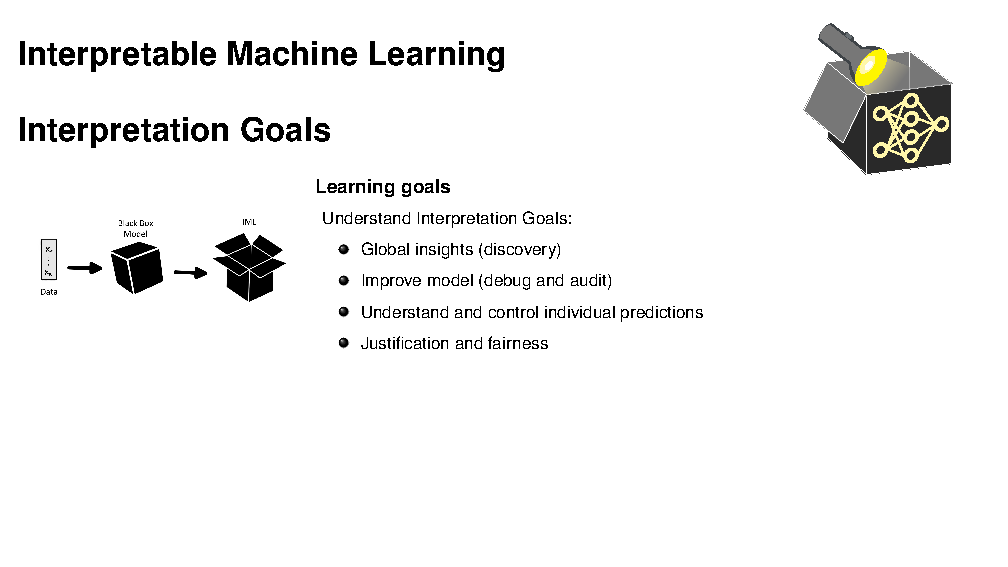
\includepdf[pages=-]{../../lecture_iml/slides-pdf/slides02-intro-goals.pdf}

%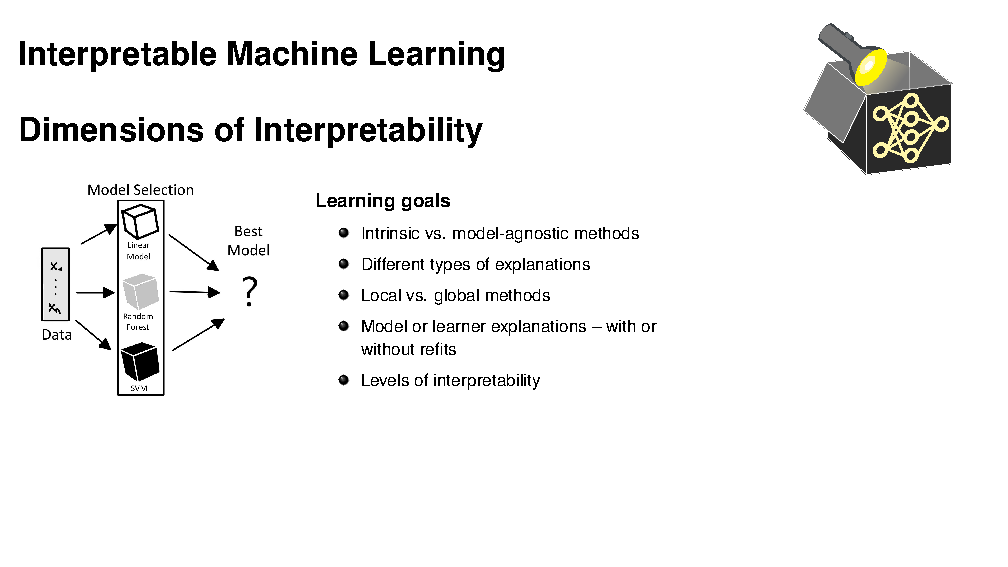
\includepdf[pages={1-13}]{../IML_pdfs_AML/slides03-intro-dimensions.pdf}
\includepdf[pages={2-4, 13}]{../IML_pdfs_AML/slides03-intro-dimensions.pdf}
%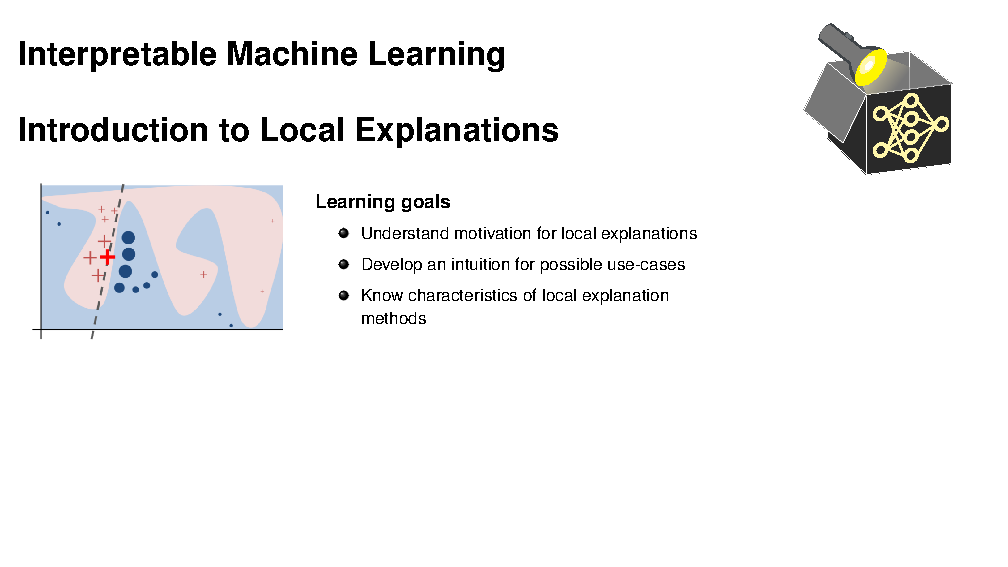
\includepdf[pages={1-7,16-21}]{../../lecture_iml/slides-pdf/slides01-le-intro.pdf}


%% LIME
\section{LIME}
\includepdf[pages={3,5, 7-last}]{../IML_pdfs_AML/slides04-le-lime.pdf}
\includepdf[pages={2-4}]{../IML_pdfs_AML/slides05-le-lime-examples.pdf}
\includepdf[pages={2}]{../IML_pdfs_AML/slides06-le-lime-pitfalls.pdf}


%% Counterfactual Explanations

\section{Counterfactual Explanations}
\includepdf[pages={2-3, 5-7,24-34}]{../IML_pdfs_AML/slides07-le-counterfactuals.pdf}
%\includepdf[pages={11-13}]{../IML_pdfs_AML/slides08-le-counterfactuals-methods.pdf}


%% INTRO FE

\section{Intro to Feature Effects}
\includepdf[pages={3-6}]{../IML_pdfs_AML/slides01-fe-intro.pdf}


%% ICE Curves

\includepdf[pages={2-10}]{../IML_pdfs_AML/slides02-fe-ice.pdf}


\end{document}